\setlength{\columnsep}{3pt}
\begin{flushleft}

\bigskip
\begin{itemize}
	\item SSH command:
	\bigskip
	\begin{tcolorbox}[breakable,notitle,boxrule=0pt,colback=pink,colframe=pink]
		\color{black}
		\fontdimen2\font=1em
		Syntax: ssh [options] [username@]remote\_server\_ip
		\fontdimen2\font=4pt
	\end{tcolorbox}
	
	\begin{figure}[h!]
		\centering
		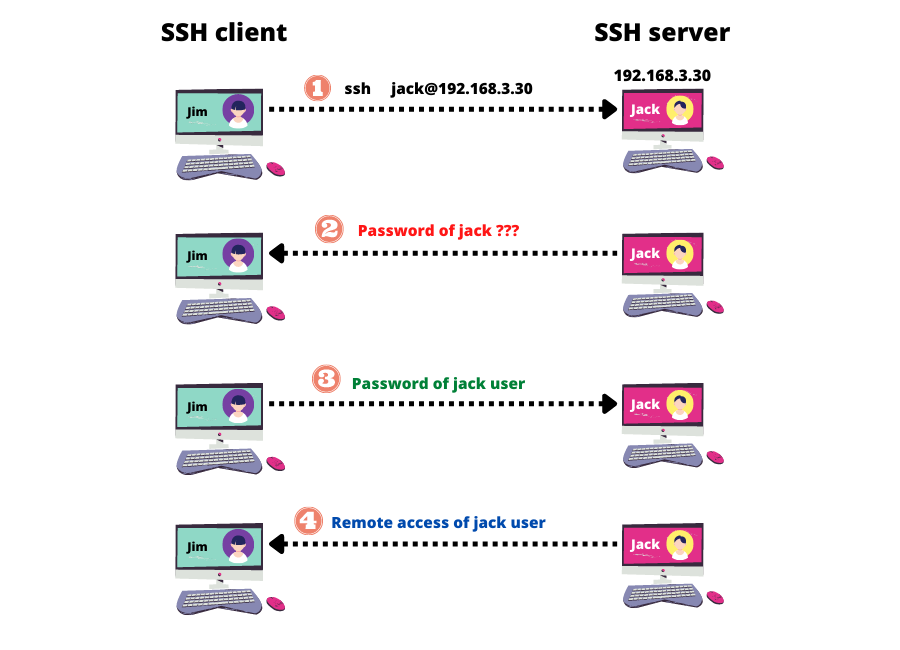
\includegraphics[scale=0.7]{content/chapter19/images/ssh_access.png}
		\caption{SSH connection using ssh command}
		\label{fig:stage5}
	\end{figure}		
	
	\newpage
	\item \textbf{Known host authentication}
	\bigskip
	\begin{itemize}
		\item The first time SSH client takes access of SSH server:
		\begin{itemize}
			\item The host public key of SSH client is stored in SSH server's \textbf{"known\_hosts"} file.
			\item This file authenticates the SSH client to the SSH server.
			\item Location of known\_host file: \textbf{{"$\sim$"}/.ssh/known\_hosts}.
		\end{itemize}
	
		\item Eg:
		\begin{figure}[h!]
			\centering
			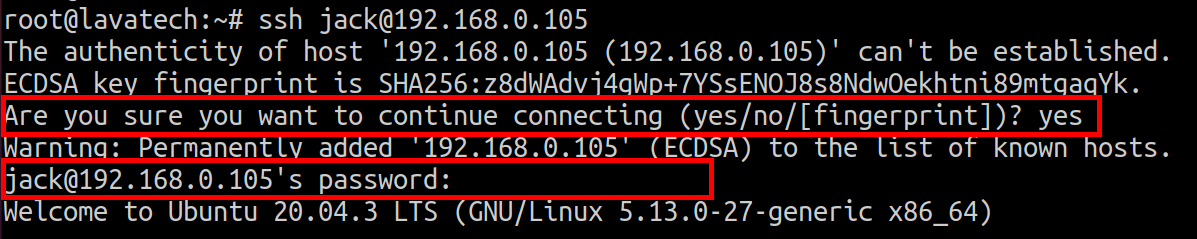
\includegraphics[scale=0.3]{content/chapter19/images/ssh6.png}
			\caption{Sample output}
			\label{fig:stage55}
		\end{figure}
		
	\end{itemize}
	\newpage
	
	\item Execute command on remote system using SSH:
		\begin{tcolorbox}[breakable,notitle,boxrule=0pt,colback=pink,colframe=pink]
		\color{black}
		\fontdimen2\font=1em
		Syntax: ssh [username@]remote\_server\_ip [command]
		\fontdimen2\font=4pt
	\end{tcolorbox}
	
	Eg:
	\begin{tcolorbox}[breakable,notitle,boxrule=-0pt,colback=black,colframe=black]
		\color{green}
		\fontdimen2\font=1em
		\# ssh jack@192.168.0.105 "logger 'Test log from remote system'"
		\fontdimen2\font=4pt
	\end{tcolorbox}
	\bigskip
	\bigskip
	
	\item Options with \textbf{ssh} command:
	\newline
	\begin{itemize}
		\item \textbf{-v}: Verbose mode to display debugging messages.Maximum 3 "v" options can be supplied.
		\begin{tcolorbox}[breakable,notitle,boxrule=0pt,colback=pink,colframe=pink]
			\color{black}
			\fontdimen2\font=1em
			Syntax: ssh -v [username@]remote\_server\_ip
			\newline
			Syntax: ssh -vv [username@]remote\_server\_ip
			\newline
			Syntax: ssh -vvv [username@]remote\_server\_ip
			\fontdimen2\font=4pt
		\end{tcolorbox}
		
		Eg:
		\begin{tcolorbox}[breakable,notitle,boxrule=-0pt,colback=black,colframe=black]
			\color{green}
			\fontdimen2\font=1em
			\# ssh -v jack@192.168.0.105
			\newline
			\# ssh -vvv jack@192.168.0.105
			\fontdimen2\font=4pt
		\end{tcolorbox}
		\bigskip
		\bigskip
		\item \textbf{-p}: Used to change port while taking remote access.
		\begin{tcolorbox}[breakable,notitle,boxrule=0pt,colback=pink,colframe=pink]
			\color{black}
			\fontdimen2\font=1em
			Syntax: ssh -p port\_number [username@]remote\_server\_ip
			\fontdimen2\font=4pt
		\end{tcolorbox}
		
		Eg:
		\begin{tcolorbox}[breakable,notitle,boxrule=-0pt,colback=black,colframe=black]
			\color{green}
			\fontdimen2\font=1em
			\# ssh -p 8080 jack@192.168.0.105
			\fontdimen2\font=4pt
		\end{tcolorbox}
		
	\end{itemize}
	
	
	
	
	
	
\end{itemize}





\end{flushleft}
\newpage


